\section{Conclusion}

\begin{frame}{Conclusion}
    \begin{itemize}
        \item Scrum offre un cadre de travail itératif et incrémental.
        \item Opposé aux méthodes classiques linéaires inadaptées.
        \item N'utilise plus les humains comme de simples ressources.
        \item Grande flexibilité face aux besoins complexes et évolutifs.
    \end{itemize}

    \pause

    \definecolor{colchall}{HTML}{B97522}
    \definecolor{colbad}{HTML}{AC3543}
    \definecolor{colgood}{HTML}{43AC35}

\vfill
\begin{columns}
    \begin{column}{.5\textwidth}
        \begin{tikzpicture}
            \draw[colgood, line width=.4cm]
                (0, 0) arc (90:39.6:1)
                node (end-1) {};

            \draw[colchall, line width=.4cm]
                (end-1) arc (39.6:-165.6:1)
                node (end-2) {};

            \draw[colbad, line width=.4cm]
                (end-2) arc (194.4:90:1);

            \node[
                align=left, anchor=center, draw=fg,
                inner sep=.5em
            ] at (-3.5, -1)
                {\textbf{Cycle en V}\\[.5em]%
                 14~\% réussite\\%
                 57~\% problèmes\\%
                 29~\% échec};
        \end{tikzpicture}
    \end{column}
    \pause
    \begin{column}{.5\textwidth}
        \begin{tikzpicture}
            \draw[colgood, line width=.4cm]
                (0, 0) arc (90:-61.2:1)
                node (end-1) {};

            \draw[colchall, line width=.4cm]
                (end-1) arc (-61.2:-237.6:1)
                node (end-2) {};

            \draw[colbad, line width=.4cm]
                (end-2) arc (122.4:90:1);

            \node[
                align=left, anchor=center, draw=fg,
                inner sep=.5em
            ] at (3.5, -1)
                {\textbf{Scrum}\\[.5em]%
                 42~\% réussite\\%
                 49~\% problèmes\\%
                 \hspace{1ex}9~\% échec};
        \end{tikzpicture}
    \end{column}
\end{columns}
\vfill

    \textbf{Source :} \url{https://www.infoq.com/articles/standish-chaos-2015}
\end{frame}

\begin{frame}{Ouvertures}
    \begin{itemize}
        \item Scrum de Scrums : passage à grande échelle.
        \item Détails du backlog : stories, epics, features, ...
        \item Intégration de Scrum avec d'autres méthodes Agiles.
    \end{itemize}

    \pause

    \vfill
    {\color{fg}\fbox{
        \begin{minipage}{.15\textwidth}
            
\includegraphics[width=1.5cm]{scrum-livre}
        \end{minipage}%
        \begin{minipage}{.75\textwidth}
            \textit{Scrum, le guide pratique de la méthode Agile la plus populaire}\\
            Claude Aubry, 4\textsuperscript{è} édition, Dunod
        \end{minipage}
    }}
\end{frame}

% Fin : sources et remerciements
\begin{frame}
    \begin{columns}
        \begin{column}{.65\textwidth}
            \begin{center}
                \LARGE
                \textbf{Merci pour votre attention~!}\\
                \Large
                N’hésitez pas à poser des questions.
            \end{center}
        \end{column}%
        \begin{column}{.35\textwidth}
            \hfill
            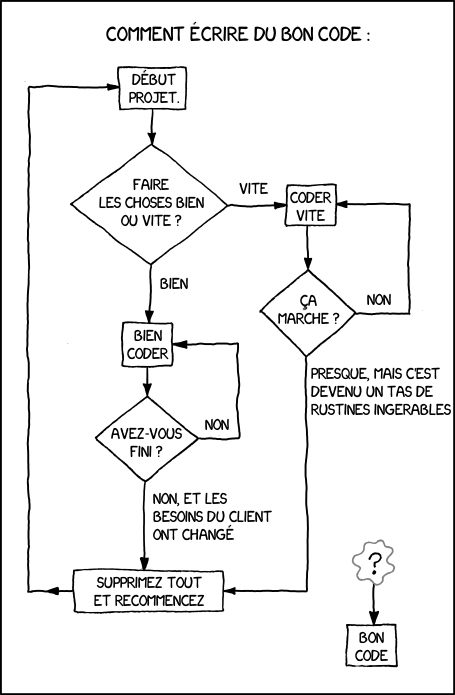
\includegraphics[height=\dimexpr\textheight-1.2cm\relax]{xkcd-fr}
        \end{column}
    \end{columns}
    \vfill
    \begin{columns}
        \begin{column}{.65\textwidth}
            {\scriptsize \textbf{Icônes :} Madebyolivier, Roundicons, Pixel Buddha, Freepik (CC 3.0 BY).}\\[-.3em]
            {\scriptsize \textbf{Arbre de la gestion de projet :} The Project Cartoon (CC 3.0 BY).}
        \end{column}%
        \begin{column}{.35\textwidth}
            \hfill{\scriptsize \textbf{Source :} XKCD (CC BY-NC 2.5)}\\[-.3em]
            \hfill{\scriptsize\url{https://xkcd.com/844/}}
        \end{column}
    \end{columns}
\end{frame}
